\chapter{Modelling of the Vehicle}\label{cha:ModelOfVehicle}

The prototype model contains software, hardware and mechanical components. Software and hardware components are easy to change and model after how the rest of the system is madded and shall run. The vehicle, which is the mechanical component, is provided to this project and therefore not changeable. This will make the functions of the vehicle, described in \secref{sec:Vehicledescription}, setup some requirements for the rest of the system. There will be madded a model of the vehicle, to described the power transfer from the motors rotational energy to the movement of the vehicle. This transfer function can be implemented in a control loop. This control loop can out from the model of the vehicle and feedback from sensors, drive the vehicle. The overall model of the vehicle model can be seen on \figref{fig:StartTotalModelsystem}.


\begin{figure}[H]
	\centering
	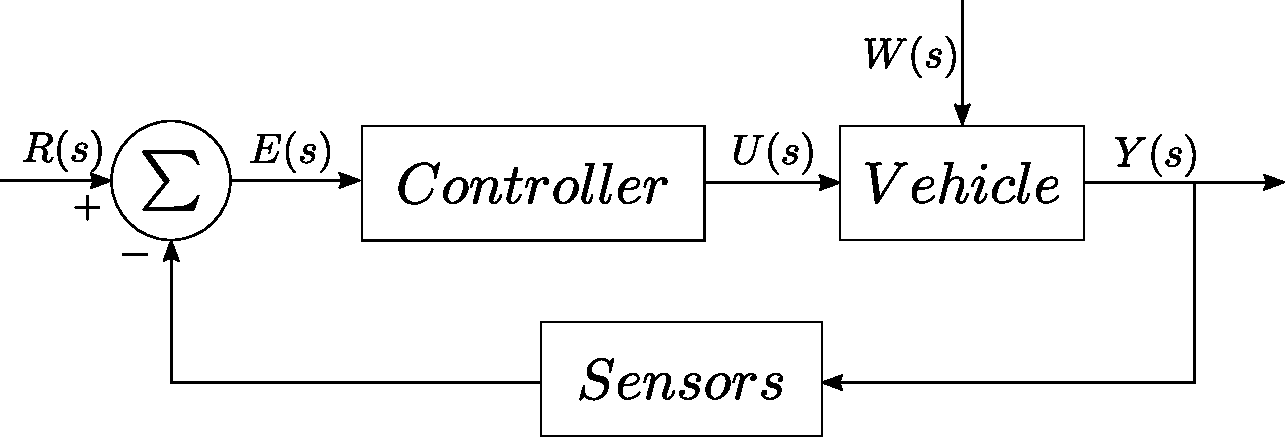
\includegraphics[scale=0.6]{figures/StartTotalModelsystem.pdf}
	\caption{A block diagram of the velocity model}
	\label{fig:StartTotalModelsystem}
\end{figure}

The input in the velocity model, $R(s)$, is the vehicle's wanted velocity and the output is the actual velocity of the vehicle. The controller receives an input, $E(s)$, which consist of the wanted speed subtracted with the actual speed measured with a sensor. Hence delivering an error which is to be corrected, to be able to achieve the wanted speed as an output. The controller should therefore deliver a voltage to the Vehicle, $U(s)$, thus, changing the rotational force of the motor and thereby changing the vehicle's velocity. The vehicle is also affected by an external disturbance, $W(s)$, e.g. a slope, wind or ground friction. The vehicles output, $Y(s)$ is the actual velocity of the vehicle. The actual velocity is measured by the sensors and subtracted from the wanted speed.

